\chapter{Background}

\label{Chapter2}

This section will present the main concepts that are relevant to the thesis project and the reason why it's useful.
It will first explain the main theory behind microservices and how it seeks to solve the main problems in legacy software architectures. Then it will
detail the new issues that arise from microservices. Finally, it will paint a picture of today's landscape of distributed software and 
tie it all together to explain the value of the research in this project.

\section{Microservices}
\subsection{The monolith}
In general when talking about both microservices and distributed computing in general, the concept of a \textbf{Monolith} often gets brought up. 
The monolith is this concept of a large, self-contained application where all the code and functionality is tightly bundled together, and is very hard to separate into individual parts.
The definition has changed over time: According to the ITS back in 2001 \cite{ITS}, a monolith was "An application in which the user interface, business rules, and data access code is combined into a single executable program and deployed on one platform."
However, most modern interpretations online refer back to a book from 2003 called \textit{The art of Unix programming}. Usually referred to as "monster monoliths", it marks the beginning of the trend of using the term monolith as a bogeyman of unmaintainable, poorly planned code. 
This trend has been continued in modern days with software "gurus" and the like when needing something to compare to our lord and savior microservices \cite*{Gouigoux2017}.
It is therefore important to remember that:
\begin{enumerate}
    \item The monolith is not a defined software architecture design paradigm. Rather, it is the default type of application that appears when not taking great effort and intentionality to split the code up in many distinct parts.
    \item The monolith is not some damnable evil to be conquered: On software projects of a less-than-huge scale, it is very often quite optimal. It doesn't have to deal with inter-component communication. Keeping everything contained in one code base makes it easy to run and test on local machines, keeps all the code in one place for easy access, and so on. 
    \item The monolith mostly just exists as a concept when talking about microservices or other ways to break it up. Its purpose is mainly to demonstrate the benefits of code splitting in large software.
\end{enumerate}

With that out of the way, let's discuss the problems with monolithic software that microservices seek to amend.

\subsection{The problems with monolithic software}
The core issue that with monolithic software is \textbf{entanglement.}
In this context, it means how complex monolithic software will have too many interconnected, interdependent parts to manage effectively.
This interdependence will mean that something that is a problem for one small part of the whole, will be a problem for the entire tech stack. \\
\\
\textbf{Scalability} refers to the ability to increase the workload capacity of the software \cite*{Scalability}. 
If the amount of users, data, geographical reach or computation complexity increases, it becomes necessary to increase hardware capabilities. 
Scaling up monolithic software can be a time-consuming and costly affair, as it usually doesn't allow for only increasing the capacity of the parts of the software that are facing increased load.  \\
An example: On the 24th of December 2004, Delta Air Lines' crew scheduling system crashed because of an integer overflow bug resulting from record system load. 
It took five days of around the clock work to implement a workaround that duplicated a database \cite*{USAToday}. 
Issues from heavy loads like this are always a risk. But entangled monolith systems are not easy to extend. 
In a microservices oriented system, implementing this extension fix would likely be on the scale of modifying a few lines of code and spinning up another instance of the database. 
I highlight this example because the fix for this huge problem ended up being a basic principle of microservices: Generating more instances of only the overloaded components. 
In summary, a microservice system is fundamentally better suited to handle scaling. 

\begin{figure}[ht] 
\centering 
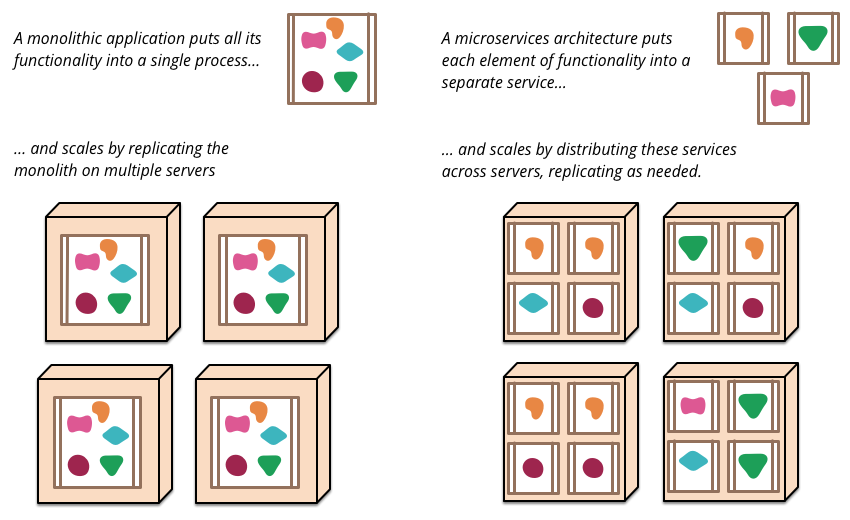
\includegraphics[width=\columnwidth]{Figures/scaling.png}
\caption{Illustrating how monoliths and microservices handle scaling. Credit: Martin Fowler \cite*{Fowler2014}}
\label{Scaling-comparison}
\end{figure}
\textbf{Comprehension} of large software is impossible. 
There is a human limit to how much one can keep in one's mind. 
In large software, the amount of functions and interactions can balloon into the tens or hundreds of thousands. 
Fully comprehending such a system is impossible for human brains, and it becomes necessary to abstract it down to a manageable mental model. 
Without good comprehension of the system, it is very difficult to make good changes, adjustments or additions.
A highly entangled monolith can very difficult to abstract, without clear boundaries for which parts do what.\\
\\
\textbf{Modern software development} is characterized by autonomous teams working separately and collaborating through continuous integration. 
This means: build often, test often, merge often. 
According to Agile practices, one should write tests first, then write code that passes the tests. 
But writing tests for highly entangled monolithic software is challenging, as even small changes can have consequences far down the chain. 
Building often will also become costly: Monolithic software will typically need to be rebuilt from scratch each time. 
A costly affair, and entirely unfeasible if the goal is to build several times a day. \\
\\
\textbf{Resilience} in the context of software has several definitions \cite*{Curtis}. 
In the context of this thesis, we can define it as "the ability to keep running correctly in spite of failures". Often called fault tolerance.
The entanglement of the monolith once again becomes a problem here. 
A single function running into an unexpected situation and throwing an error will, by default in most technologies, abort the execution of the program entirely.
It can be circumvented by try/catch statements and other error handling methods, but an entangled system is extremely difficult to make fault tolerant. \\
\\
\textbf{Updating and technical debt.} As the monolith grows, making any change becomes a larger project.
The more entangled everything is, the more changes will have to be made to accommodate updated dependencies or changes in behavior. 
These changes to accommodate the change can also cause other things to be changed.
This can lead to mounting technical debt: As updating components is such a project, it is delayed.
But each delay leads to an increase in how big of a project it would be to properly update dependencies.
